%%%%%%%%%%%%%%%%%%%%%%%%%%%%%%%%%%%%%%%%%%%%%%%%%%%%%%%%%%%%%%%%%%%%%%%%%%%%%%%%
\documentclass[11pt]{article} % Dokumentenklasse

\usepackage[utf8]{inputenc} % Textkodierung: UTF-8
\usepackage[T1]{fontenc} % Zeichensatzkodierung

\usepackage[USenglish]{babel}% http://ctan.org/pkg/babel
\usepackage{graphicx} % Grafiken
\usepackage[absolute]{textpos} % Positionierung

% Schriftart Helvetica:
\usepackage[scaled]{helvet}
\renewcommand{\familydefault}{\sfdefault}

\usepackage{calc} % Berechnungen
\usepackage{tabto} % Tabulatoren
\usepackage{parskip}

\usepackage{enumitem}

% Debugging:
%\usepackage{layout} % Layout-Informationen
%\usepackage{printlen} % Längenwerte ausgeben

%%%%%%%%%%%%%%%%%%%%%%%%%%%%%%%%%%%%%%%%%%%%%%%%%%%%%%%%%%%%%%%%%%%%%%%%%%%%%%%%
% EINSTELLUNGEN
%%%%%%%%%%%%%%%%%%%%%%%%%%%%%%%%%%%%%%%%%%%%%%%%%%%%%%%%%%%%%%%%%%%%%%%%%%%%%%%%

% Seitenränder:
\newcommand{\SeitenrandOben}{43.5mm}
\newcommand{\SeitenrandRechts}{20mm}
\newcommand{\SeitenrandLinks}{20mm}
\newcommand{\SeitenrandUnten}{10mm}

\newcommand{\UniversitaetLogoBreite}{19mm}
\newcommand{\UniversitaetLogoHoehe}{1cm}

\usepackage[a4paper,
top=\SeitenrandOben,
bottom=\SeitenrandUnten,
inner=\SeitenrandLinks,
outer=\SeitenrandRechts,
foot=0cm,
head=0cm
]{geometry}

\textblockorigin{\SeitenrandLinks}{\SeitenrandOben} % Ursprung für Positionierung

\setlength{\parindent}{0pt}
%\setlength{\baselineskip}{32pt}
\setlength{\parskip}{\baselineskip}
\TabPositions{4cm}
\pagestyle{empty}

%%%%%%%%%%%%%%%%%%%%%%%%%%%%%%%%%%%%%%%%%%%%%%%%%%%%%%%%%%%%%%%%%%%%%%%%%%%%%%%%
% General stuff
%%%%%%%%%%%%%%%%%%%%%%%%%%%%%%%%%%%%%%%%%%%%%%%%%%%%%%%%%%%%%%%%%%%%%%%%%%%%%%%%
\newcommand{\Problem}[1]{\paragraph*{Problem #1:}\qquad}
\newcommand{\Topic}[1]{
	\newpage
	\section*{#1}}

\newcommand{\Given}{\textbf{Given:\qquad\qquad}}
\newcommand{\Searched}{\textbf{Searched:\qquad}}
\newcommand{\Solution}{\textbf{Solution:\qquad}}

%%%%%%%%%%%%%%%%%%%%%%%%%%%%%%%%%%%%%%%%%%%%%%%%%%%%%%%%%%%%%%%%%%%%%%%%%%%%%%%%
% Math stuff
%%%%%%%%%%%%%%%%%%%%%%%%%%%%%%%%%%%%%%%%%%%%%%%%%%%%%%%%%%%%%%%%%%%%%%%%%%%%%%%%
\usepackage{amsmath}
\usepackage{amssymb}

\newcommand{\R}{\mathbb{R}}
\newcommand{\Vector}[1]{\R^{#1}}
\newcommand{\Matrix}[2]{\R^{#1 \times #2}} % !!! DON'T TOUCH !!!
%%%%%%%%%%%%%%%%%%%%%%%%%%%%%%%%%%%%%%%%%%%%%%%%%%%%%%%%%%%%%%%%%%%%%%%%%%%%%%%%


\newcommand{\ExerciseNumber}{07}

\newcommand{\PersonOne}{Marcel Bruckner (03674122)}
\newcommand{\PersonTwo}{Julian Hohenadel (03673879)}
\newcommand{\PersonThree}{Kevin Bein (03707775)}


%%%%%%%%%%%%%%%%%%%%%%%%%%%%%%%%%%%%%%%%%%%%%%%%%%%%%%%%%%%%%%%%%%%%%%%%%%%%%%%%
% DOKUMENT
%%%%%%%%%%%%%%%%%%%%%%%%%%%%%%%%%%%%%%%%%%%%%%%%%%%%%%%%%%%%%%%%%%%%%%%%%%%%%%%%

\begin{document}

%%%%%%%%%%%%%%%%%%%%%%%%%%%%%%%%%%%%%%%%%%%%%%%%%%%%%%%%%%%%%%%%%%%%%%%%%%%%%%%%
\begin{textblock*}{\UniversitaetLogoBreite}[1,0](\textwidth-1mm, 2cm-\SeitenrandOben)%
	\raggedleft
\includegraphics{../Ressources/Universitaet_Logo_RGB.pdf}%
\end{textblock*}


\begin{textblock*}{\textwidth}[0,0](0cm, 0cm)%
	{\fontsize{24pt}{26pt}\selectfont\textbf{Exercise}}
	
	\vspace*{14pt}
	{\fontsize{18pt}{27pt}\selectfont\textbf{\ExerciseNumber}}
\end{textblock*}

\vspace*{92.2mm}
\fontsize{15pt}{17.5pt}\selectfont%
TUM Department of Informatics

\renewcommand{\baselinestretch}{1.47}
\normalsize\selectfont
\vspace*{17.1mm}
\textbf{Supervised by}\tab
\begin{minipage}[t]{\textwidth-\CurrentLineWidth}
	Prof. Dr. Stephan Günnemann\\
	Informatics 3 - Professorship of Data Mining and Analytics\strut
\end{minipage}

\vspace*{4.3mm}
\textbf{Submitted by}\tab
\begin{minipage}[t]{\textwidth-\CurrentLineWidth}
	\PersonOne\\
	\PersonTwo\\
	\PersonThree
\end{minipage}

\vspace*{-1mm}
\textbf{Submission date}\tab 
\begin{minipage}[t]{\textwidth-\CurrentLineWidth}
	Munich, \today
\end{minipage}
\newpage % !!! DON'T TOUCH !!!
%%%%%%%%%%%%%%%%%%%%%%%%%%%%%%%%%%%%%%%%%%%%%%%%%%%%%%%%%%%%%%%%%%%%%%%%%%%%%%%%

%%%%%%%%%%%%%%%%%%%%%%%%%%%%%%%%%%%%%%%%%%%%%%%%%%%%%%%%%%%%%%%%%%%%%%%%%%%%%%%%
% !!! HOMEWORK STARTS HERE !!!
%%%%%%%%%%%%%%%%%%%%%%%%%%%%%%%%%%%%%%%%%%%%%%%%%%%%%%%%%%%%%%%%%%%%%%%%%%%%%%%%
%
\Topic{Constrained Optimization}
%
\Problem{1}
%
\begin{flushleft}
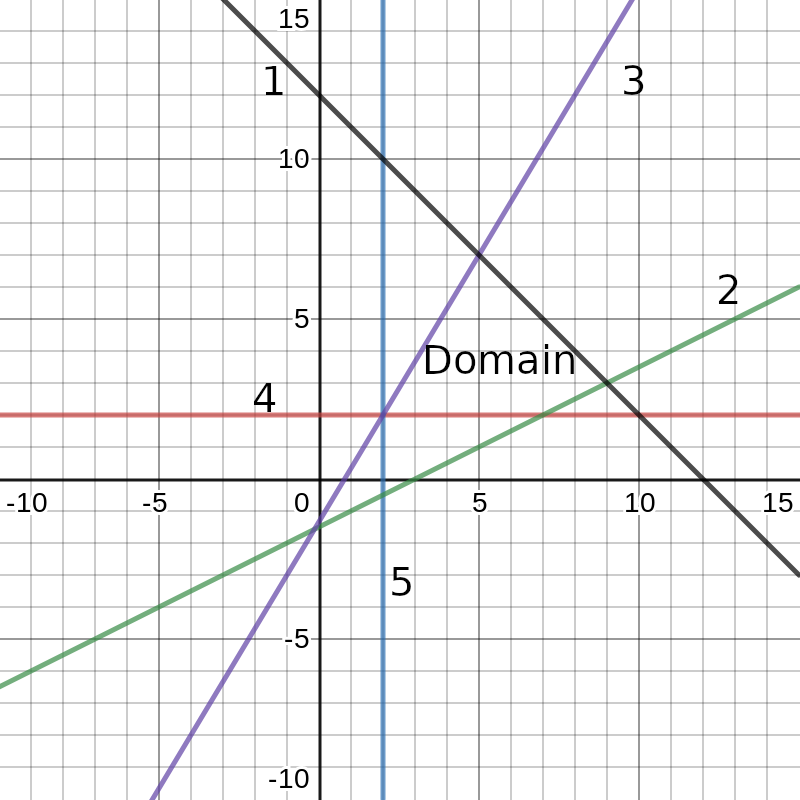
\includegraphics[width=0.7\textwidth]{problem1.png}
\end{flushleft}
\begin{flushleft}
Since $f_0$ is a hyperplane, the min and max values are at the vertices:
\end{flushleft}
\begin{align*}
  f_0((9,3)^T) = -2 \;\;\;\;\;& f_0((5,7)^T) = -11 \\ f_0((7,2)^T) = 8 \;\;\;\;\;& f_0((9,3)^T) = 9
\end{align*}
\begin{flushleft}
  We immediately see that $\theta_\text{min} = (5,7)^T$ and $\theta_\text{max} = (9,3)^T$ and also $\mathrm{min}(f_0) = -11$ and $\mathrm{max}(f_0) = 9$.
\end{flushleft}
%
%
\newpage
\Problem{2}
%
\begin{flushleft}
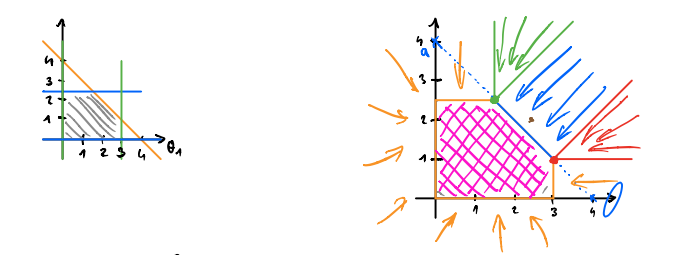
\includegraphics[width=0.7\textwidth]{problem2.png}
\end{flushleft}
\begin{equation*}
  \pi_\chi(p) = 
  \begin{cases}
    {\color{magenta}p} & {\color{magenta}\text{if } p\in \chi} \\
    {\color{forestgreen}(1.5,2.5)^T} & {\color{forestgreen}\text{if $p$ is in the green corridor}} \\
    {\color{red}(3,1)^T} & {\color{red}\text{if $p$ is in the red corridor}} \\
    {\color{blue}\begin{pmatrix}
      \frac{1}{2} p_1 - \frac{1}{2} p_2 + 2 \\
      \frac{1}{2} - p_1 + \frac{1}{2} p_2 + 2 \\
    \end{pmatrix}} & {\color{blue}\text{if $p$ is in the blue corridor}} \\
    {\color{orange}\begin{pmatrix}
      \mathrm{max}(0, \mathrm{min}(3, p_1)) \\
      \mathrm{max}(0, \mathrm{min}(2.5, p_2))
    \end{pmatrix}} & {\color{orange}\text{if $p$ is outside green/red/blue corridor and } p \not\in \chi}
    \end{cases} 
\end{equation*}
\begin{flushleft}
The blue corridor projects down to a line. We can take any two points on the line to calculate the projection vector $\pi_{\chi_{a,b}}$. We choose $\mathbf{a}:=(0,4)^T$ and $\mathbf{b}:=(4,0)^T$ for simplicity.
\end{flushleft}
\begin{align*}
  \pi_{\chi_{a,b}} &= a + \frac{(\mathbf{p} - \mathbf{a})^T (\mathbf{b} - \mathbf{a})}{\Vert \mathbf{b} - \mathbf{a} \Vert^2_2} (\mathbf{b} - \mathbf{a})  \\
  &= \left(\begin{smallmatrix}0 \\ 4 \end{smallmatrix}\right) + \frac{\left(\begin{smallmatrix}p_1 - 0 \\ p_2 - 4 \end{smallmatrix}\right)^T \left(\begin{smallmatrix}4 \\ -4 \end{smallmatrix}\right)}{32} \left(\begin{smallmatrix}4 \\ -4 \end{smallmatrix}\right) \\
  &= \left(\begin{smallmatrix}0 \\ 4 \end{smallmatrix}\right) + \frac{4p_1 - 4p_2 + 16}{32} \left(\begin{smallmatrix}4 \\ -4 \end{smallmatrix}\right) \\
  &= \left(\begin{smallmatrix}0 \\ 4 \end{smallmatrix}\right) + \left(\frac{1}{8} p_1 - \frac{1}{8} p_2 + \frac{1}{2} \right) \left(\begin{smallmatrix}4 \\ -4 \end{smallmatrix}\right) \\
  &=\begin{pmatrix}
      \frac{1}{2} p_1 - \frac{1}{2} p_2 + 2 \\
      \frac{1}{2} - p_1 + \frac{1}{2} p_2 + 2 \\
    \end{pmatrix}
\end{align*}
%
%
\newpage
\Problem{3}
%
\begin{flushleft}
1. Formulate the Lagrangian:
\begin{align*}
  L(\theta, \alpha) &= f_0(\theta) + \sum^M_{i=1} \alpha_i f_i(\theta) \\
  &= \theta_1 - \sqrt{3} \theta_2 + \alpha(\theta_1^2  + \theta_2^2 - 4) \\
  &= \theta_1 - \sqrt{3} \theta_2 + \alpha\theta_1^2 + \alpha\theta_2^2 - \alpha 4
\end{align*}
2.1 Solve:
\begin{align*}
  g(\alpha) &= \underset{\theta}{\min}\left[ L(\theta, \alpha)\right] \\
  &= \underset{\theta}{\min}\left[\theta_1 - \sqrt{3} \theta_2 + \alpha \theta_1^2 + \alpha \theta_2^2 - \alpha 4 \right] \\
  &\Rightarrow \left[ \theta_1 - \sqrt{3} \theta_2 + \alpha \theta_1^2 + \alpha \theta_2^2 - \alpha 5 \right]' \overset{!}{=} 0 \\
  &\Rightarrow \nabla_\theta L(\mathbf{\theta}, \alpha) =
  \begin{pmatrix}
    1 + 2 \alpha \theta_1 \\
    - \sqrt{3} + 2 \alpha \theta_2
  \end{pmatrix} = \overset{!}{=} 0 \\
  &\Rightarrow \begin{cases}
    1 + 2 \alpha \theta_1 = 0 \\
    -\sqrt{3} + 2 \alpha \theta_2 = 0
  \end{cases} \\
  &\Rightarrow \begin{cases}
    \theta_1 = -\frac{1}{2\alpha} \\
    \theta_2 = \frac{\sqrt{3}}{2 \alpha}
  \end{cases}
\end{align*}
2.2 Get the dual function $g(\alpha)$:
\begin{align*}
  g(\alpha) &= L(\theta, \alpha) \\
  &= \theta_1 - \sqrt{3} \theta_2 + \alpha \theta_1^2 + \alpha \theta^2 - \alpha 4 \\
  &= -\frac{1}{2 \alpha} - \sqrt{3} \frac{\sqrt{3}}{2 \alpha} + \alpha \left( -\frac{1}{2 \alpha} \right)^2 + \alpha \left( \frac{\sqrt{3}}{2 \alpha} \right)^2 - \alpha 4 \\
  &= -\frac{1}{2 \alpha} - \frac{3}{2 \alpha} + \left(\frac{1}{4 \alpha} \right) + \left(\frac{3}{4 \alpha} \right) - \alpha 4 \\
  &= - \frac{1}{\alpha} - \alpha 4 
\end{align*}
3. Solve the dual problem:
\[ 
\left[g(\alpha)\right]' = \frac{1}{\alpha^2} - 4 \Rightarrow \alpha = \frac{1}{2} \text{ (since $\alpha \geq 0$)}
\]
\[ 
g\left(\frac{1}{2}\right) = -4
\]
Slater's condition holds.
\end{flushleft}
\begin{flushleft}
The minimizer $\theta$ becomes:
\end{flushleft}
\[ \theta_1 = -\frac{1}{2\alpha} = -\frac{1}{2\cdot\frac{1}{2}} = -1 \]
\[ \theta_2 = \frac{\sqrt{3}}{2 \alpha} = \frac{\sqrt{3}}{2 \cdot \frac{1}{2}} = \sqrt{3} \]
%
%
\newpage
\Problem{4}
%
\begin{flushleft}
Since the constrained $f_i(\theta)$ must be less or equal to 0 for $i=1,\ldots,N$ we first reformulate it:
\[ 1 - y_i(\mathbf{w}^T \mathbf{x}_i + b) \leq 0 \]
Next we can set up the Lagrangian: 
\[ L(\mathbf{w}, b, \mathbf{\alpha}) = \frac{1}{2} \mathbf{w}^T\mathbf{w} + \sum_{i=1}^N \alpha_i (1 - y_i(\mathbf{w}^T \mathbf{x}_i + b)) \]
and obtain the dual function $g(\alpha) = \underset{w,b}{\min} L(\mathbf{w},b,\mathbf{\alpha})$ by solving $\nabla_{\mathbf{w},b} L(\mathbf{w},b,\mathbf{\alpha}) = 0$:
\end{flushleft}
\begin{align*}
  \nabla_{\mathbf{w},b} L(\mathbf{w},b,\mathbf{\alpha}) &= \nabla_{\mathbf{w},b} \frac{1}{2} \mathbf{w}^T\mathbf{w} + \sum_{i=1}^N \alpha_i y_i \mathbf{w}^T \mathbf{x}_i + \alpha_i y_i + b \\
  &= \begin{pmatrix} \mathbf{w} + \sum_{i=1}^N \alpha_i (-y_i) \mathbf{x}_i \\ \sum_{i=1}^N \alpha_i y_i \end{pmatrix} \overset{!}{=} 0 \\
  &\Rightarrow w = \sum_{i=1}^N \alpha_i y_i \mathbf{x}_i \;\;\text{ and }\;\; \sum_{i=1}^N \alpha_i y_i = 0
\end{align*}
\begin{flushleft}
Substitute $w$ back into $L$ to get $g(\alpha)$:
\end{flushleft}
\begin{align*}
g(\alpha) &= \frac{1}{2} \sum_{i=1}^N \alpha_i y_i \mathbf{x}_i^T \sum_{j=1}^N \alpha_j y_j \mathbf{x}_j + \sum_{i=1}^N \alpha_i \left( 1 - y_i \left( \sum_{j=1}^N \alpha_j y_j \mathbf{x}_j^T \mathbf{x}_i + b \right) \right) \\
&= -\frac{1}{2} \sum_{i=1}^N\sum_{j=1}^N \alpha_i \alpha_j y_i y_j \mathbf{x}_i^T \mathbf{x}_j + \sum_{i=1}^N \alpha_i
\end{align*}
\begin{flushleft}
The dual problem is therefore:
\end{flushleft}
\begin{align*}
\text{maximize } & g(\alpha) = \sum_{i=1}^N \alpha_i - \frac{1}{2} \sum_{i=1}^N\sum_{j=1}^N \alpha_i \alpha_j y_i y_j \mathbf{x}_i^T \mathbf{x}_j \\
\text{subject to } & \sum_{i=1}^N \alpha_i y_i = 0 \\
& \alpha_i \geq 0 \text{ for } i=1,\ldots,N
\end{align*}
\begin{flushleft}
Since this is a quadratic programming problem, all $f_i(\theta)$ are \textit{convex} ($\Rightarrow$ bounded from below) and since $\alpha_i \geq 0$, $\alpha$ is \textit{feasible}. This makes the duality gap zero and so strong duality holds.
\end{flushleft}

%
%
%%%%%%%%%%%%%%%%%%%%%%%%%%%%%%%%%%%%%%%%%%%%%%%%%%%%%%%%%%%%%%%%%%%%%%%%%%%%%%%%
% !!! HOMEWORK ENDS HERE !!!
%%%%%%%%%%%%%%%%%%%%%%%%%%%%%%%%%%%%%%%%%%%%%%%%%%%%%%%%%%%%%%%%%%%%%%%%%%%%%%%%

%%%%%%%%%%%%%%%%%%%%%%%%%%%%%%%%%%%%%%%%%%%%%%%%%%%%%%%%%%%%%%%%%%%%%%%%%%%%%%%%
\newpage

\vspace*{-15.8mm}
\fontsize{19pt}{21pt}\selectfont

\vspace{25.3mm}
Appendix

\normalsize\selectfont
\vspace{13.2mm}
We confirm that the submitted solution is original work and was written by us without further assistance. Appropriate credit has been given where reference has been made to the work of others.

\vspace{18.1mm}
\rule[-3.7mm]{\linewidth}{0.5pt}
Munich, \today, Signature \PersonOne

\vspace{18.1mm}
\rule[-3.7mm]{\linewidth}{0.5pt}
Munich, \today, Signature \PersonTwo

\vspace{18.1mm}
\rule[-3.7mm]{\linewidth}{0.5pt}
Munich, \today, Signature \PersonThree
 % !!! DON'T TOUCH !!!
%%%%%%%%%%%%%%%%%%%%%%%%%%%%%%%%%%%%%%%%%%%%%%%%%%%%%%%%%%%%%%%%%%%%%%%%%%%%%%%%

\end{document}
